% Created 2015-09-14 Mon 00:57
\documentclass{scrartcl}
\usepackage[utf8]{inputenc}
\usepackage[T1]{fontenc}
\usepackage{fixltx2e}
\usepackage{graphicx}
\usepackage{longtable}
\usepackage{float}
\usepackage{wrapfig}
\usepackage{soul}
\usepackage{textcomp}
\usepackage{marvosym}
\usepackage{wasysym}
\usepackage{latexsym}
\usepackage{amssymb}
\usepackage{hyperref}
\tolerance=1000
\usepackage[margin=18mm]{geometry}
\usepackage{amsmath}
\usepackage{graphicx}
\usepackage{subfigure}
\usepackage{parskip}
\usepackage{standalone}
\usepackage{tikz,pgf,pgfplots}
\usetikzlibrary{decorations.pathmorphing,patterns}
\usetikzlibrary{arrows,snakes,backgrounds,patterns,matrix,shapes,fit,calc,shadows,plotmarks,decorations.markings,datavisualization,datavisualization.formats.functions,intersections,external}
\usetikzlibrary{decorations.pathmorphing,patterns}
\pgfplotsset{compat=1.9}
\newcommand*{\mexp}[1]{\ensuremath{\mathrm{e}^{#1}}}
\newcommand*{\laplace}[1]{\ensuremath{\mathcal{L} \{#1\}}}
\newcommand*{\laplaceinv}[1]{\ensuremath{\mathcal{L}^{-1} \{#1\}}}
\newcommand*{\realpart}[1]{\ensuremath{\operatorname{Re}(#1)}}
\newcommand*{\impart}[1]{\ensuremath{\operatorname{Im}(#1)}}
\newcommand*{\vsp}[1]{\rule{0pt}{#1}}
\newcommand*{\tderiv}[1]{\ensuremath{\frac{d^{#1}}{dt^{n}}}}
\newcommand*{\bbm}{\begin{bmatrix}}
\newcommand*{\ebm}{\end{bmatrix}}
\newcommand*{\obsmatrix}{\mathcal{O}}
\newcommand*{\contrmatrix}{\mathcal{C}}
\newcommand*{\cwh}{\ensuremath{\cos \omega h}}
\newcommand*{\swh}{\ensuremath{\sin \omega h}}
\newcommand*{\zethree}{\big(z - \mexp{-3h}\big)}
\providecommand{\alert}[1]{\textbf{#1}}

\title{Computerized control - partial exam 1 (dummy)}
\author{Kjartan Halvorsen}
\date{Due 2015-09-18}
\hypersetup{
  pdfkeywords={},
  pdfsubject={},
  pdfcreator={Emacs Org-mode version 7.9.3f}}

\begin{document}

\maketitle



\section*{Problem 1}
\label{sec-1}

Consider the continuous-time system with the following transfer function
\[ G(s) = \frac{s+1}{s(s+3)}. \]
The system is sampled with sampling interval $h$ using zero-order hold. \textbf{Show that the pulse-transfer function for the sampled system is}
\[ H(z) = \frac{(2z-2+3h)\zethree{} - 2(z-1)^2}{9(z-1)\zethree{}}. \]
\section*{Problem 2}
\label{sec-2}

  The sampled system in Problem 1 is controlled using proportional control with gain equal to 1. 
  \begin{center}
  \includestandalone[width=0.5\linewidth]{feedback}
  \end{center}

\begin{enumerate}
\item Calculate the closed-loop pulse-transfer function
\item Let $h=\frac{\ln 2}{3} \approx 0.23$. Is the closed-loop system stable?
\end{enumerate}
\section*{Solutions}
\label{sec-3}
\subsection*{Problem 1}
\label{sec-3-1}

   First calculate the step-response of the continous-time system
   \[G(s)\frac{1}{s} = \frac{s+1}{s^2(s+3)} = \frac{2}{9s} + \frac{1}{3s^2} - \frac{2}{9(s+3)}.\]
   The inverse Laplace-transform gives
   \[ y(t) = \frac{2}{9} + \frac{1}{3}t - \frac{2}{9}\mexp{-3t}. \]
   Sampling this function gives
   \[ y(kh) = \frac{2}{9} + \frac{1}{3}kh - \frac{2}{9}\big(\mexp{-3h}\big)^k, \]
   which has the Z-transform
   \[Y(z) = \frac{2z}{9(z-1)} + \frac{hz}{3(z-1)^2} - \frac{2z}{9\zethree{}}. \]
   Dividing the z-transform of the system response to that of the input (the step) gives
   \begin{align*}
   H(z) &= \frac{Y(z)}{U(z)} = \frac{z-1}{z}Y(z) = \frac{2}{9} + \frac{h}{3(z-1)} - \frac{2(z-1)}{9\zethree{}}\\
        &= \frac{2(z-1)\zethree{} + 3h\zethree{} - 2(z-1)^2}{9(z-1)\zethree{}}\\
        &= \frac{(2z-2+3h)\zethree - 2(z-1)^2}{9(z-1)\zethree{}}.
   \end{align*}
\subsection*{Problem 2}
\label{sec-3-2}


\begin{enumerate}
\item The closed loop system becomes
      \begin{align*}
          H_c(z) &= \frac{H(z)}{1+H(z)}\\
                 &= \frac{(2z-2+3h)\zethree{} - 2(z-1)^2}{(2z-2+3h)\zethree{} - 2(z-1)^2+9(z-1)\zethree{}}\\
                 &= \frac{(2z-2+3h)\zethree{} - 2(z-1)^2}{(2z-2+3h+9z-9)\zethree{} - 2(z-1)^2}\\
                 &= \frac{(2z-2+3h)\zethree{} - 2(z-1)^2}{(11z+3h-11)\zethree{} - 2(z-1)^2}
      \end{align*}
\item Stability of the closed-loop system. Substituting $h=\frac{\ln2}{3}$ gives the characteristic equation
      \[ (11z + \ln2 - 11)\big(z-\frac{1}{2}\big) - 2z^2 +4z - 2
           = 9z^2 - (12.5-\ln2)z + 3.5 - 0.5\ln 2 = 0. \]
      Apply Jury's  criterion:


\begin{center}
\begin{tabular}{llll}
 $9$                                   &  $-11.81$                                      &  $3.15$  &                                                \\
 $3.15$                                &  $-11.81$                                      &  $9$     &  $\alpha_2 = \frac{3.15}{9}$                   \\
\hline
 $9-\frac{3.15^2}{9}\approx 7.9$       &  $-11.81 + \frac{3.15}{9}11.81 \approx -7.68$  &          &                                                \\
 $-7.68$                               &  $7.9$                                         &          &  $\alpha_1 = -\frac{7.68}{7.9} \approx -0.97$  \\
\hline
 $7.9 - 0.96 \cdot 7.68 \approx 0.44$  &                                                &          &                                                \\
\end{tabular}
\end{center}



      The first element in each odd row in the table are positive $\Rightarrow$ \textbf{The closed loop system is stable.}

      Step response (not asked for):
      \begin{center}
      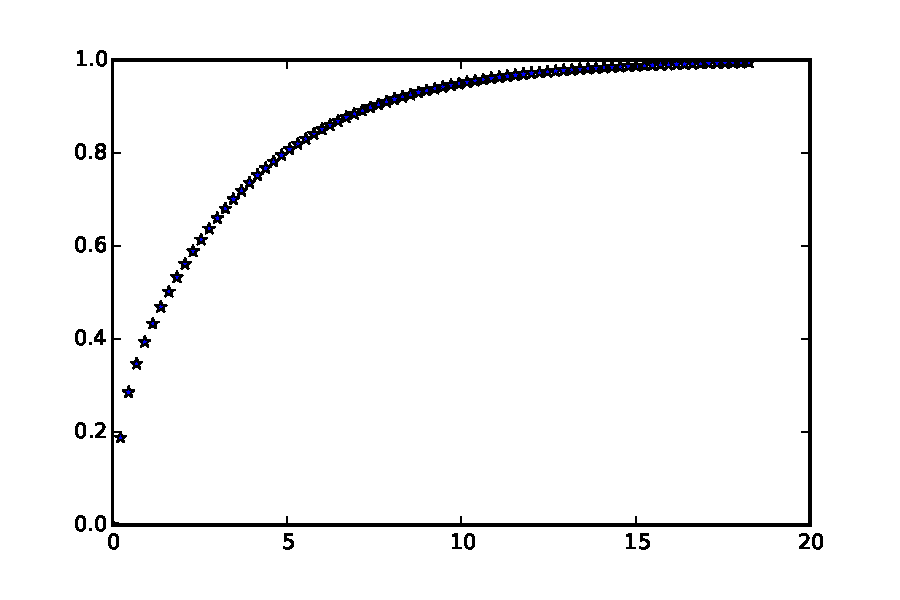
\includegraphics[width=0.7\linewidth]{stepresponse}
      \end{center}
\end{enumerate}

\end{document}
